\documentclass[a4paper]{jsarticle}
\usepackage[all]{xy}
\usepackage[dvipdfmx]{graphicx}
\usepackage{../math_note, exercise, enumitem}
\renewcommand{\thesection}{Ex7.\arabic{section}}

\newcommand{\coverU}{\mathfrak{U}}
\newcommand{\coverV}{\mathfrak{V}}

\newcommand{\Div}{\operatorname{Div}}
\newcommand{\Cl}{\operatorname{Cl}}
\newcommand{\CaCl}{\operatorname{CaCl}}
\newcommand{\nullCaCl}{\operatorname{CaCl}^{0}}
\newcommand{\Pic}{\operatorname{Pic}}

\begin{document}
    以下での($*$)とは,次のもの:
    \begin{itemize}
        \item integral,
        \item separated,
        \item noetherian, and
        \item regular in codimention one.
    \end{itemize}

    また,($\dagger$)は次のもの:
    $X$ :: noetherian scheme, 
    $\shS$ :: graded $\shO_X$-algebra
    となっている.
    また,$d \in \Z, d \geq 0$について,
    $\shS_d$ :: homogeneous part of $\shS$を$U \mapsto \shS(U)_d$.
    $X,\shS$は次をすべて満たす.
    \begin{itemize}
        \item $\shS$ :: quasi-coherent.
        \item $\shS=\bigoplus_{d \geq 0} \shS_d$.
        \item $\shS_0=\shO_X$.
        \item $\shS_1$ :: coherent $\shO_X$-module.
        \item $\shS$ :: locally generated by $\shS_1$ as $\shO_X$-algebra.
    \end{itemize}

\section{Surjective Mophism between Invertible Sheaves is Isomorphic.} %% Ex7.1 
    $X$ :: locally ringed space,
    $\shL, \shM$ :: invertible sheaves on $X$,
    $f: \shL \to \shM$ :: surjective mophism,
    とする.
    
    \paragraph{Proof 1.}
    任意の点$x \in X$をとり,$A=\shO_{X,x}$とおく.
    $f_x: \shL_x \to \shM_x$は同型写像を合成することで
    $\phi: A \to A$ :: surjective $A$-morphismと同一視出来る.
    $\phi$ :: surjectiveより,
    $\phi(\alpha)=1 \in A$となる$\alpha \in A$がとれる.
    また$\phi$は$A$-module morphismだから,$\alpha \phi(1)=1$.
    そこで$\psi: A \to A$を$a \mapsto \alpha a$と定義すれば,
    これが$\phi$の逆写像になる.
    よって$\phi, f_x$は同型.
    Prop1.1から,$f$ :: iso.

    \paragraph{Proof 2.}
    Matsumura, Thm2.4から分かる.
    これはNAK (or Nakayama's Lemma)からの帰結である.

    \begin{Remark}
        $k(x)$ :: residue fieldと
        $f_x: \shL_x \to \shM_x$をテンソルすると,
        $f_x \otimes \id{k(x)}$ :: surjective $k(x)$-module morphismが得られる.
        よって$\ker (f_x \otimes \id{k(x)})=0$.
        しかし,ここからNAKをつかって$\ker f_x=0$を導くことは出来ない.
        $k(x)$がflat $\shO_{X,x}$-moduleでなく,
        したがって$\ker (f_x \otimes \id{k(x)})$と$(\ker f_x) \otimes k(x)$の間に同型があることが
        言えないからである.
        このことはflat $\implies$ torsion-freeに気をつければすぐに分かる.
        同様の議論が$f_x$ :: injective(と$\coker f_x$)の場合に出来ることにも気づくが,
        このときは$\Z_2 \to \Z_2; 1 \mapsto 3$という反例がある.
    \end{Remark}

\section{Two Sets of Global Generators and Corresponding Morphisms.} %% Ex7.2 
    $k$ :: field,
    $X$ :: scheme /$k$,
    $\shL$ :: invertible sheaf on $X$,
    $S=\{s_0,\dots,s_m\}, T=\{t_0,\dots,t_n\}$ :: global generators of $\shL$.
    とする.
    ここで$S,T$は
    同じ線形(部分)空間$V \subseteq \Gamma(X, \shL)$を張るとする.
    また$n \leq m, d=\dim_k V$とする.

    $S,T$からそれぞれThm7.1のように定まるmorphismを$\phi_S, \phi_T$とする.
    $\phi_S$が次のように分解できることを示す.
    \[
        \xymatrix
        {
            X \ar@/_20pt/[rrrr]_-{\phi_S}\ar[r]^-{\phi_T}&
                \im \phi_T \ar@{^{(}->}[r]& \proj^m-L \ar[r]^-{\pi}&
                    \proj^n \ar[r]^-{\alpha}& \proj^n
        }
    \]
    ここで$\pi, \alpha$はそれぞれlinear projectionとautomorphismである.

    $X \to \proj^n$のmorphismを考えることは,
    $k[y_0,\dots, y_n]$の元$y_0,\dots,_n$の変換を考えることと同じである.
    これはThm7.1の証明を観察すれば分かる.
    二つの$k$-linear mapは$\phi_S^*, \phi_T^*$はそれぞれ,
    $y_i \mapsto s_i (i=0,\dots,n)$,
    $y_i \mapsto t_i (i=0,\dots,m)$で定まっている.
    したがって問題は,
    $t_0,\dots,t_m$を$s_0,\dots,s_n$へ
    変換するprojectionとautomorphismをつくる問題,
    と言い換えられる.

    今,次のような$(m+1) \times (n+1)$行列$Q$が存在する.
    \[
        \tatev{ s_0 \\ \vdots \\ s_n }
        =Q \tatev{ t_0 \\ \vdots \\ t_m }.
    \]
    $S,T$が$V$の生成系であることから$\rank Q=\dim V=:d$.
    $Q$は基本行列をいくつもかける(あるいは基本変形を繰り返し行う)ことにより,
    次の形に分解できる.
    \[
        Q=L P_{d} R~~
        \mwhere~ L \in PGL(m,k), R \in PGL(n,k)
    \]
    ただし行列$P_r ~(r=1,\dots,n+1)$は$r \times r$-identity matrix $I_r$をもちいて
    $P_{r}=
    \begin{bmatrix}
        I_r & 0 \\
        0 & 0
    \end{bmatrix}$
    と定義される行列である.
    (TODO: $P_{d}$を$P_{n+1}$に交換しても問題ない?)
    $L, P_{n+1}, R$が誘導するmorphismをそれぞれ$\beta, \tilde{\pi} ,\alpha$とすれば,
    $\alpha, \beta$はautomorphismであり,
    $\tilde{\pi}$はprojectionである.
    \[
        \xymatrix
        {
            \proj^m \ar[r]^-{\beta}& \proj^m
            \ar@{^{(}->}[r]^-{i}& \proj^m-L
            \ar[r]^-{\tilde{\pi}}& \proj^n
            \ar[r]^-{\alpha}& \proj^n
        }
    \]
    求める写像はこの$\alpha$と,$\pi=\beta \circ i \circ \tilde{\pi}$である.
    また,$L=\zerosp(y_0,\dots,y_n) \subseteq \proj^m$の次元は$m-(n+1)$である.

\section{Morphism of $\proj^n \to \proj^m$ can be Decomposed into Common Ones.} %% Ex7.3
    $\phi: \proj^n_k \to \proj^m_k$を考える.
    $\shO_{\proj^m}(1), \shO_{\proj^n}(1)$
     :: invertible sheaves
    のglobal generatorをそれぞれ
    $\{x_0,\dots,x_m\}, \{y_0,\dots,y_n\}$
    とする.

    \subsection{$\im \phi=pt$ or $m \geq n$ and $\dim \im \phi=n$.}
%    $\eta: \Gamma(\proj^m, \shO_{\proj^m}(1)) \to \Gamma(\proj^m, \phi^* \phi_* (\shO_{\proj^m}(1)))$を
%    adjoint pair $\phi^* \dashv \phi_*$のunitから得られる写像とする.
%    これが本文中で$\phi^*$と表記されているものである
    $s_i=\phi^*(x_i)~(i=0,\dots,m)$とおくと,
    $s_0,\dots,s_m$は$\shL:=\phi^*(\shO_{\proj^m}(1))$のglobal generatorである.
    $\shL$は$\proj^n$上のinvertible sheafだから,
    Cor6.17より,$\shL \iso \shO_{\proj^n}(d)$となる$d \in \Z$が存在する.
    Example7.8.3同様,$\shO_{\proj^n}(d)$は$|d|$次斉次単項式で生成される.

    \paragraph{$m<n \implies \dim \im \phi=0$.}
    \paragraph{$m \geq n \implies \dim \im \phi=n$.}

\section{If $X$ Admits an Ample Invertible Sheaf, then $X$ is Separated.} %% Ex7.4
    \subsection{Assumption of Thm7.6 $\implies$ $X$ :: separated.}
    $A$ :: noetherian ring,
    $X$ :: scheme of finite type /$A$とする.
    $\shL$ :: ample invertible sheaf on $X$が存在したとする.
    Thm7.6から,immersion $i: X \to \proj^n_A ~(n>0)$が存在する.
    これは$X$から$\proj^n_A$のlocally closed subschemeへのisomorphismである.
    これにprojection $\pr: \proj^n_A=\proj^n_{\Z} \times_{\Z} \Spec A \to \Spec A$を
    合成したものは,quasi-projective.
    \[\xymatrix
    {
        X \ar[r]^-{\sim}& U \cap Z~ \ar@{^{(}->}[r]& \proj^n_A \ar[r]^-{\pr}& \Spec A
    }\]
    $U, Z$はそれぞれ$\proj^n_A$のopen, closed subschemeである.
    $A,X$についての仮定から$\Spec A, X$ :: noetherian schemeがわかる
    \footnote
    {
        $f: X \to \Spec A$がfinite typeならば
        $f^{-1}\Spec A=X$はfinite affine open coverをもち,
        各affine open coverはfinitely generated $A$-algebraの$\Spec$である.
        finitely generated $A$-algebraは$A$からnoetherianを受け継ぐから,
        $X$ :: noetherian.
    }
    から,
    Thm4.9より,この写像$X \to \Spec A$はseparated.
    
    \subsection{There is No Ample Invertible Sheaf on 
        \protect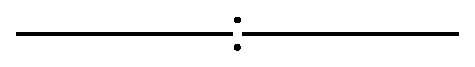
\includegraphics[width=2.5cm]{./images/affine_with_doubled_origin.eps} / a field $k$.}
    $k$ :: field,
    $X$ :: affine with doubled origin /$k$とする.
    より詳細に,$X$は$X_1=\Spec k[x], X_2=\Spec k[y]$を
    $U_1=X_1-\{O_1\}, U_2=X_2-\{O_2\}$で貼りあわせたものとする.
    ただし$O_1 \in X_1,O_2 \in X_2$は原点である.
    $X_i, U_i, O_i ~~(i=1,2)$はすべて$X$の部分集合とみなす.
    $X$ :: noetherian integral schemeは明らか.
    Example 6.3.1, Cor 6.16より,$\Pic X_1, \Pic X_2=0$.

    まず$\Pic X$を計算する.
    $\shL \in \Pic X$をとる.
    $X_{12}:=X_1 \cap X_2 (\iso \affine^1-\{0\})$としておく.
    %% Lemma5.3, Prop5.4を見ながら考えると,
    %% \shLはaffine open coverへのrestriction
    %% $(\shL|_{X_1}, \shL|_{X_2})$で定まると分かる.
    %% $\shL|_{X_{12}}$は以下のように$x^n$で定まり,
    %% Lemma5.3から,これは$\shL|_{X_1}$も定める.
    %% $\shL|_{X_1}=(x^{-n}k[x])\sidetilde, \shL|_{X_2}=(k[y])\sidetilde$となり,
    %% 確かにこれらの$X_{12}$への制限は(単元倍を除いて)一致する.
    $\Pic X_{12}=0$ (Prop6.2, Cor6.16)より,
    $\shO_{X_{12}} \iso \shL|_{X_{12}}$.
    さらに$X_{12}$は$D(x) \subseteq \Spec k[x]$と同型であるから,
    \[ \shO_{X_{12}}=\shO_{X_1}|_{X_{12}}=(k[x]_x)\sidetilde=(k[x,x^{-1}])\sidetilde. \]
    すなわち$\Gamma(X_{12},\shO_{X_{12}})=k[x,x^{-1}]$.
    $X_{12}$はaffineだから,Ex5.3より,
    $\shO_{X_{12}} \isomap \shL|_{X_{12}}$は
    $k[x,x^{-1}] \isomap \Gamma(X_{12}, \shL|_{X_{12}})$の
    $k[x,x^{-1}]$-isomorphismによって決定される.
    この同型射は$k[x,x^{-1}]$の単元をかける写像によって定まる.
    そして単元は$a x^n ~(a \in k^*, n \in \Z)$と書ける.
    また,$k^*=\Gamma(X_{12},\shO_{X_{12}}^*)$の分の違いは無視されるから,
    結局同型射は$x^n ~(n \in \Z)$で定まる.
    こうして,$\shO_{X_{12}} \isomap \shL|_{X_{12}}$が$\Z$に対応することが分かった.
    この同型射で$\shL$全体も定まる(??).
    以上から$\Pic X \iso \Z$.

    $n \in \Z$に対応する$\Pic X$の元を$\shL_n$と書く.
    $\Pic X \iso \CaCl X$に注意して,
    $\shL_n$に対応するCarier Divisorを考えると,
    これは$\{\sect{U_1}{x^{-n}}, \sect{U_2}{1} \}$である.

    $\shL_n$がglobal generatorを持つのは$n=0$
    すなわち$\shL_n=\shO_X$であるときのみ.
    $\shL_0 \otimes \shL_n \iso \shL_n$なので,
    ample sheafは存在しない.
    \url{ https://math.stackexchange.com/questions/70042 }.
          
\section{ Ample and Very Ample are Inherted by Tensor Products.} %% Ex7.5 
          
\section{The Riemann-Roch Problem.} %% Ex7.6 

\section{Some Rational Surfaces.} %% Ex7.7 

\section{Sections of $\pi: \P(\shE) \to X$
    $\leftrightarrow$ Quotient Invertible Sheaves of $\shE$.} %% Ex7.8 

\section{ } %% Ex7.9 

\section{$P^n$-Bundles Over a Scheme.} %% Ex7.10 

\section{Different Sheaves of Ideals can Give Rise to Isomorphic Blow Up Schemes.} %% Ex7.11 

\section{ } %% Ex7.12 

\section{* A Complete Nonprojective Variety.} %% Ex7.13 

\section{ } %% Ex7.14 


\end{document}
